%==============================================================================
% WebGPU "mezzanine" GPU offload of the ns-3 contrib/nr 3GPP channel model
% Short, intuitive talk (~10 min). Build: latexmk -pdf main.tex (see README.md)
%==============================================================================
\documentclass[aspectratio=169,11pt]{beamer}

% --- Theme: metropolis if available, graceful fallback to Madrid -------------
\IfFileExists{beamerthememetropolis.sty}{%
  \usetheme{metropolis}
  \metroset{numbering=fraction,progressbar=frametitle,block=fill}
}{%
  \usetheme{Madrid}\usecolortheme{seahorse}
}

\usepackage[T1]{fontenc}
\usepackage[utf8]{inputenc}
\usepackage{amsmath,amssymb}
\usepackage{booktabs}
\usepackage{colortbl}
\usepackage{tikz}
\usepackage{pgfplots}
\pgfplotsset{compat=1.17}
\usetikzlibrary{arrows.meta,positioning,fit,backgrounds,calc}

\definecolor{cpuCol}{RGB}{200,80,60}
\definecolor{gpuCol}{RGB}{50,120,190}
\definecolor{mezCol}{RGB}{40,150,110}
\definecolor{warnCol}{RGB}{210,150,30}
\definecolor{boxgray}{RGB}{235,235,235}

\tikzset{
  stage/.style={draw,rounded corners,thick,align=center,minimum height=8mm,
                font=\scriptsize,fill=boxgray},
  gpu/.style={stage,draw=gpuCol,fill=gpuCol!12},
  cpu/.style={stage,draw=cpuCol,fill=cpuCol!12},
  mez/.style={stage,draw=mezCol,fill=mezCol!15},
  flow/.style={-{Stealth[length=2.4mm]},thick},
  lab/.style={font=\tiny\itshape,align=center,text=black!60},
  mat/.style={draw,thick,fill=gpuCol!18},
  vecc/.style={draw,thick,fill=mezCol!20},
  pol/.style={draw,thick,fill=warnCol!25},
}

\newcommand{\code}[1]{\texttt{\small #1}}

\title{Running the 5G Channel Model on a GPU}
\subtitle{A WebGPU ``mezzanine'' for the ns-3 / nr 3GPP (TR 38.901) channel}
\author{ns-3 \texttt{spectrum} + contrib/nr}
\date{\today}

\begin{document}

\maketitle

%==============================================================================
\begin{frame}{What the channel model actually computes}
  \begin{columns}[c]
  \begin{column}{0.55\textwidth}
    A base station (gNB) sends radio to phones (UEs). Walls and ground
    \alert{reflect and scatter} it, so many copies arrive at once.
    \vspace{0.6em}
    \begin{block}{The model's job}
      For every link, work out \alert{how strong and how clean} the signal is --
      the \alert{SINR} (signal vs.\ interference + noise).
    \end{block}
    \vspace{0.4em}
    {\small That single number hides a \alert{lot} of arithmetic. Here is why.}
  \end{column}
  \begin{column}{0.43\textwidth}
    \centering
    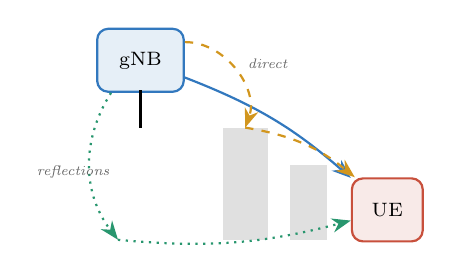
\begin{tikzpicture}[scale=0.95]
      \node[gpu,minimum width=11mm] (bs) at (0,2.4) {gNB};
      \draw[thick] (0,2.0)--(0,1.5);
      \fill[black!12] (1.1,0) rectangle (1.7,1.5);
      \fill[black!12] (2.0,0) rectangle (2.5,1.0);
      \node[cpu,minimum width=9mm] (ue) at (3.3,0.4) {UE};
      \draw[flow,gpuCol] (bs) to[bend left=10] (ue);
      \draw[flow,warnCol,dashed] (bs) to[bend left=55] (1.4,1.5);
      \draw[flow,warnCol,dashed] (1.4,1.5) to[bend left=15] (ue);
      \draw[flow,mezCol,dotted] (bs) to[bend right=35] (-0.3,0);
      \draw[flow,mezCol,dotted] (-0.3,0) to[bend right=10] (ue);
      \node[lab] at (1.7,2.35) {direct};
      \node[lab] at (-0.9,0.9) {reflections};
    \end{tikzpicture}\\[0.3em]
    {\scriptsize multipath: many routes at once}
  \end{column}
  \end{columns}
\end{frame}

%==============================================================================
\begin{frame}{Where these computations sit in the 5G NR link}
  \centering
  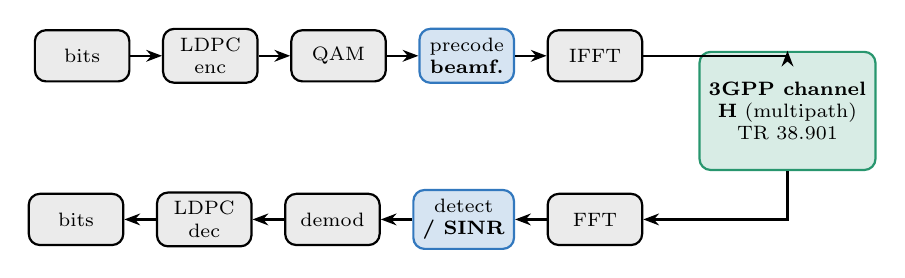
\begin{tikzpicture}[
    blk/.style={draw,rounded corners,thick,align=center,minimum height=6.5mm,
                minimum width=12mm,font=\scriptsize,fill=boxgray},
    hot/.style={blk,draw=gpuCol,fill=gpuCol!20},
    fl/.style={-{Stealth[length=2mm]},thick},
    node distance=3.5mm and 4mm]
    % --- Tx chain (top, left to right) ---
    \node[blk] (bits) {bits};
    \node[blk,right=of bits] (enc) {LDPC\\enc};
    \node[blk,right=of enc] (mod) {QAM};
    \node[hot,right=of mod] (bf) {precode\\\textbf{beamf.}};
    \node[blk,right=of bf] (ifft) {IFFT};
    \foreach \a/\b in {bits/enc,enc/mod,mod/bf,bf/ifft} \draw[fl] (\a)--(\b);
    % --- channel (right, bridging the two rows) ---
    \node[draw,thick,rounded corners,draw=mezCol,fill=mezCol!18,align=center,
          font=\scriptsize,minimum height=15mm,minimum width=20mm,
          right=7mm of ifft,yshift=-7mm] (chan)
      {\textbf{3GPP channel}\\\textbf{H} (multipath)\\\scriptsize TR 38.901};
    \draw[fl] (ifft.east) -| (chan.north);
    % --- Rx chain (bottom, right to left) ---
    \node[blk,below=14mm of ifft] (fft) {FFT};
    \node[hot,left=of fft] (det) {detect\\\textbf{/ SINR}};
    \node[blk,left=of det] (dem) {demod};
    \node[blk,left=of dem] (dec) {LDPC\\dec};
    \node[blk,left=of dec] (out) {bits};
    \draw[fl] (chan.south) |- (fft.east);
    \foreach \a/\b in {fft/det,det/dem,dem/dec,dec/out} \draw[fl] (\a)--(\b);
  \end{tikzpicture}
  \vspace{0.3em}
  \begin{itemize}\small
    \item The \textcolor{mezCol}{\textbf{channel H}} (multipath, Eq.\ 7.5-22) is the
          billions-of-products block -- the mezzanine's main job.
    \item \textcolor{gpuCol}{\textbf{Beamforming}} (Tx) and the
          \textcolor{gpuCol}{\textbf{per-link SINR}} (Rx, incl.\ the MIMO
          interference covariance) ride on the same GPU pass.
    \item Coding / modulation / FFT are \alert{cheap} -- they stay on the CPU.
  \end{itemize}
\end{frame}

%==============================================================================
\begin{frame}{One SINR value = a chain of matrix $\times$ vector products}
  \centering
  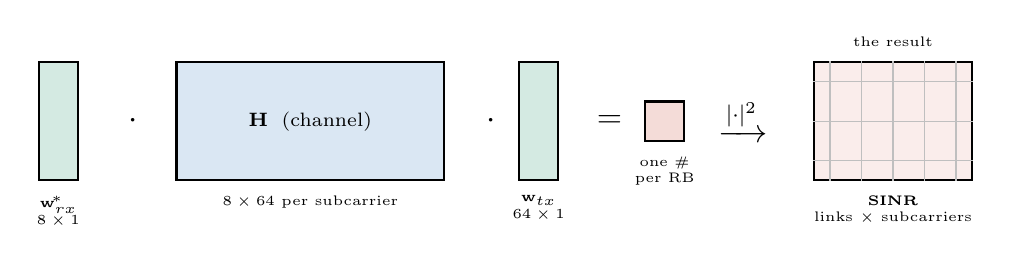
\begin{tikzpicture}[every node/.style={font=\scriptsize}]
    % --- main beamforming chain ---
    \node[vecc,minimum width=5mm,minimum height=15mm] (wrx) at (0,0) {};
    \node[below=0.6mm of wrx,font=\tiny,align=center] {$\mathbf{w}_{rx}^{\!*}$\\$8\times1$};
    \node[font=\large] (d1) at (0.95,0) {$\cdot$};
    \node[mat,minimum width=34mm,minimum height=15mm] (H) at (3.2,0)
        {\textbf{H} \;(channel)};
    \node[below=0.6mm of H,font=\tiny] {$8\times64$ per subcarrier};
    \node[font=\large] (d2) at (5.5,0) {$\cdot$};
    \node[vecc,minimum width=5mm,minimum height=15mm] (wtx) at (6.1,0) {};
    \node[below=0.6mm of wtx,font=\tiny,align=center] {$\mathbf{w}_{tx}$\\$64\times1$};
    \node[font=\large] (eq) at (7.0,0) {$=$};
    \node[draw,thick,fill=cpuCol!20,minimum width=5mm,minimum height=5mm] (sc) at (7.7,0) {};
    \node[below=0.6mm of sc,font=\tiny,align=center] {one \#\\per RB};
    \node[font=\large] at (8.7,0) {$\xrightarrow{|\cdot|^2}$};
    % --- SINR grid ---
    \node[draw,thick,fill=cpuCol!10,minimum width=20mm,minimum height=15mm] (grid) at (10.6,0) {};
    \foreach \x in {-0.8,-0.4,0,0.4,0.8} \draw[black!25] ([xshift=\x cm]grid.north)--([xshift=\x cm]grid.south);
    \foreach \y in {-0.5,0,0.5} \draw[black!25] ([yshift=\y cm]grid.west)--([yshift=\y cm]grid.east);
    \node[below=0.6mm of grid,font=\tiny,align=center] {\textbf{SINR}\\links $\times$ subcarriers};
    \node[above=0.6mm of grid,font=\tiny] {the result};
  \end{tikzpicture}

  \vspace{0.9em}
  {\scriptsize\itshape and every entry of \textbf{H} is itself a tiny sandwich (TR 38.901 Eq.\ 7.5-22):}\\[0.4em]
  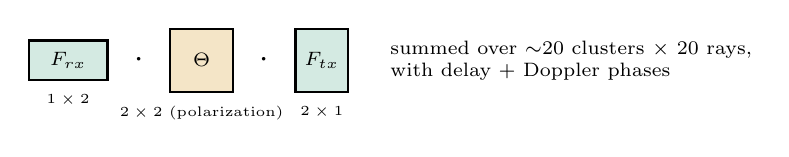
\begin{tikzpicture}[every node/.style={font=\scriptsize}]
    \node[vecc,minimum width=10mm,minimum height=5mm] (frx) {$F_{rx}$};
    \node[below=0.4mm of frx,font=\tiny] {$1\times2$};
    \node[font=\large,right=2mm of frx] (m1) {$\cdot$};
    \node[pol,minimum width=8mm,minimum height=8mm,right=2mm of m1] (th) {$\Theta$};
    \node[below=0.4mm of th,font=\tiny] {$2\times2$ (polarization)};
    \node[font=\large,right=2mm of th] (m2) {$\cdot$};
    \node[vecc,minimum width=5mm,minimum height=8mm,right=2mm of m2] (ftx) {$F_{tx}$};
    \node[below=0.4mm of ftx,font=\tiny] {$2\times1$};
    \node[right=4mm of ftx,align=left] (sum)
      {summed over \alert{$\sim$20 clusters $\times$ 20 rays},\\
       with delay + Doppler phases};
  \end{tikzpicture}
\end{frame}

%==============================================================================
\begin{frame}{Now multiply the counts -- that is the whole problem}
  To fill \alert{one} H entry, for \alert{one} link, at \alert{one} subcarrier:
  \vspace{0.3em}
  \begin{center}\small
  \begin{tabular}{rl}
    $8\times64$ antenna pairs & $=512$ tiny $2{\times}2$ products\\
    $\times\ 20$ clusters $\times\ 20$ rays & $\approx 2\times10^{5}$ products / subcarrier\\
    $\times\ \sim\!273$ subcarriers & $\approx 5.6\times10^{7}$ products / link\\
    $\times$ thousands of links & $\approx$ \alert{tens of billions}\\
    $\times$ redrawn every $\sim$100\,ms & \alert{again, and again, and again}\\
  \end{tabular}
  \end{center}
  \vspace{0.4em}
  \begin{block}{Punchline}
    A coverage map or a system simulation is \alert{billions of tiny matrix
    products}, repeated every channel update. That is what we want to move off
    the CPU.
  \end{block}
\end{frame}

%==============================================================================
\begin{frame}{Why a GPU}
  All those tiny products are \alert{the same arithmetic on independent data}.
  \vspace{0.4em}
  \begin{columns}[T]
  \begin{column}{0.48\textwidth}
    \centering\textbf{\textcolor{cpuCol}{CPU}}: one link at a time\\[0.4em]
    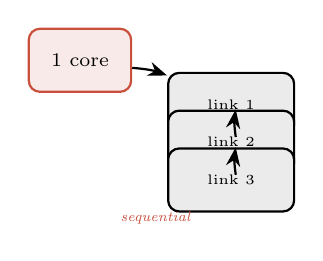
\begin{tikzpicture}[scale=0.8]
      \node[cpu,minimum width=13mm] (c) at (0,2.2) {1 core};
      \foreach \i/\y in {1/1.5,2/0.9,3/0.3} \node[stage,minimum width=16mm,font=\tiny] (l\i) at (2.4,\y) {link \i};
      \draw[flow] (c) to[bend left=8] (l1);
      \draw[flow] (l1) to[bend left=8] (l2);
      \draw[flow] (l2) to[bend left=8] (l3);
      \node[lab,text=cpuCol] at (1.2,-0.3) {sequential};
    \end{tikzpicture}
  \end{column}
  \begin{column}{0.48\textwidth}
    \centering\textbf{\textcolor{gpuCol}{GPU}}: thousands at once\\[0.4em]
    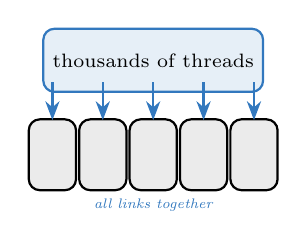
\begin{tikzpicture}[scale=0.8]
      \node[gpu,minimum width=24mm] (g) at (0,2.4) {thousands of threads};
      \foreach \x in {-1.6,-0.8,0,0.8,1.6} \node[stage,minimum width=6mm,minimum height=9mm,font=\tiny] at (\x,0.9) {};
      \foreach \x in {-1.6,-0.8,0,0.8,1.6} \draw[flow,gpuCol] (\x,2.05)--(\x,1.45);
      \node[lab,text=gpuCol] at (0,0.1) {all links together};
    \end{tikzpicture}
  \end{column}
  \end{columns}
  \vspace{0.5em}
  {\small \alert{Catch:} you need enough parallel work. A tiny job can still be
  faster on the CPU -- we hit exactly that once (last slide).}
\end{frame}

%==============================================================================
\begin{frame}{The ``mezzanine'': run the whole 3GPP chain on the GPU}
  A thin layer \alert{between} ns-3 and the GPU. Same data in and out -- nothing
  downstream changes.
  \vspace{0.5em}
  \begin{center}
  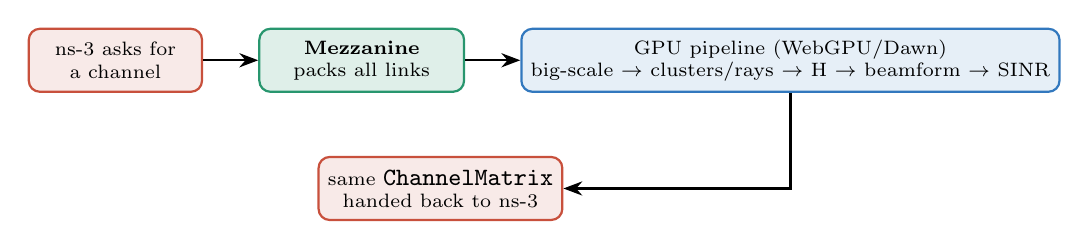
\begin{tikzpicture}[node distance=5mm and 7mm]
    \node[cpu,minimum width=22mm] (api) {ns-3 asks for\\a channel};
    \node[mez,minimum width=26mm,right=of api] (mz) {\textbf{Mezzanine}\\packs all links};
    \node[gpu,minimum width=46mm,right=of mz] (gpu)
      {GPU pipeline (WebGPU/Dawn)\\\scriptsize big-scale $\to$ clusters/rays
       $\to$ H $\to$ beamform $\to$ SINR};
    \node[cpu,minimum width=24mm,below=8mm of mz,xshift=10mm] (back)
      {same \code{ChannelMatrix}\\handed back to ns-3};
    \draw[flow] (api)--(mz); \draw[flow] (mz)--(gpu);
    \draw[flow] (gpu.south) |- (back.east);
  \end{tikzpicture}
  \end{center}
  \begin{itemize}\small
    \item The kernels were ported from \alert{CUDA to WebGPU} (WGSL shaders).
    \item Rule we held to: the \alert{heavy compute stays on the GPU} -- no
          sneaky CPU fallback.
    \item \alert{Element-exact}: feed the GPU's draw back through the CPU model
          and the matrices match to single-precision noise.
  \end{itemize}
\end{frame}

%==============================================================================
\begin{frame}{Where the parallelism lives: one Tx, many links, one GPU pass}
  \centering
  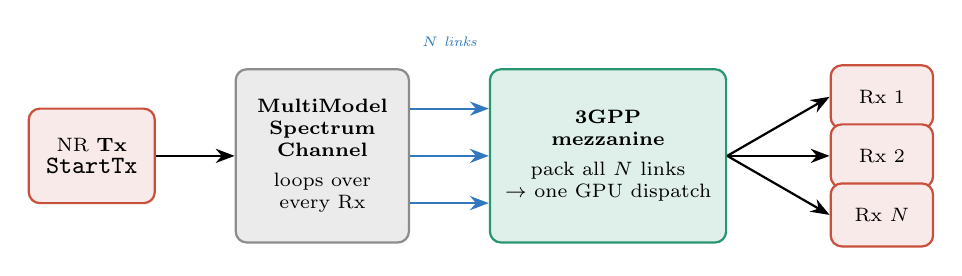
\begin{tikzpicture}[node distance=7mm and 10mm,font=\scriptsize]
    \node[cpu,minimum width=16mm,minimum height=12mm] (tx) {NR \textbf{Tx}\\\code{StartTx}};
    \node[stage,draw=black!45,minimum width=22mm,minimum height=22mm,right=of tx,align=center]
         (mm) {\textbf{MultiModel}\\\textbf{Spectrum}\\\textbf{Channel}\\[1mm]
               \scriptsize loops over\\\alert{every Rx}};
    \node[mez,minimum width=30mm,minimum height=22mm,right=of mm,align=center]
         (mez) {\textbf{3GPP}\\\textbf{mezzanine}\\[1mm]\scriptsize pack \alert{all $N$ links}\\
                $\to$ \alert{one} GPU dispatch};
    \node[cpu,minimum width=13mm,right=13mm of mez,yshift=7.5mm]  (r1) {Rx 1};
    \node[cpu,minimum width=13mm,right=13mm of mez]              (r2) {Rx 2};
    \node[cpu,minimum width=13mm,right=13mm of mez,yshift=-7.5mm] (rN) {Rx $N$};
    \draw[flow] (tx)--(mm);
    \foreach \dy in {6,0,-6} \draw[flow,gpuCol] ([yshift=\dy mm]mm.east)--([yshift=\dy mm]mez.west);
    \draw[flow] (mez.east)--(r1.west);
    \draw[flow] (mez.east)--(r2.west);
    \draw[flow] (mez.east)--(rN.west);
    \node[lab,text=gpuCol] at ($(mm.east)!0.5!(mez.west)+(0,1.45)$) {$N$ links};
  \end{tikzpicture}
  \vspace{0.3em}
  \begin{columns}[T]
  \begin{column}{0.5\textwidth}
    \begin{block}{Axis 1 -- across links (already there)}\scriptsize
      \code{MultiModelSpectrumChannel::StartTx} fans \alert{one} Tx out to
      \alert{every} Rx. On the CPU that is $N$ \alert{sequential} channel calls;
      the mezzanine packs all $N$ into \alert{one} GPU job.
    \end{block}
  \end{column}
  \begin{column}{0.5\textwidth}
    \begin{block}{Axis 2 -- inside each link}\scriptsize
      Every H is itself parallel: GPU threads $=$
      \alert{links $\times$ clusters $\times$ rays $\times$ Tx$\cdot$Rx elements
      $\times$ subcarriers} -- billions of independent products.
    \end{block}
  \end{column}
  \end{columns}
  \vspace{0.2em}
  {\scriptsize At \code{EndRx} the per-receiver MIMO \alert{interference covariance}
   is \alert{deferred} and the whole slot's receivers run in \alert{one more} GPU
   dispatch -- the batch lever (next).}
\end{frame}

%==============================================================================
\begin{frame}{Did we get the same answer? -- show, don't tell}
  \begin{columns}[c]
  \begin{column}{0.54\textwidth}
    \centering
    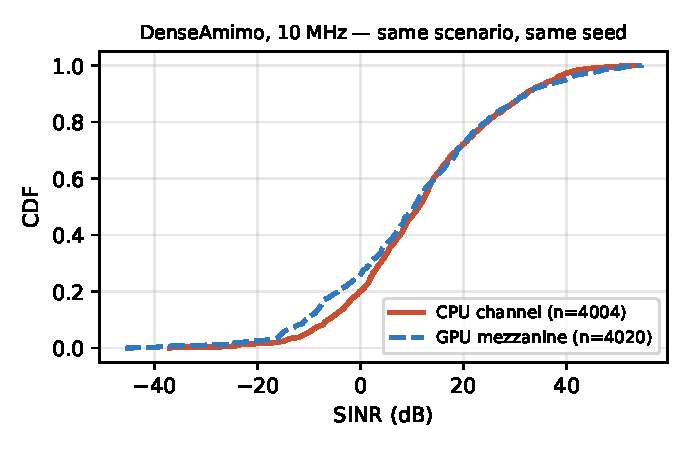
\includegraphics[width=\textwidth]{fig-sinr-cdf.pdf}
  \end{column}
  \begin{column}{0.44\textwidth}\small
    Same scenario, same seed --\\ \textcolor{cpuCol}{CPU channel} vs
    \textcolor{gpuCol}{GPU mezzanine}.
    \begin{itemize}
      \item The SINR CDFs \alert{sit on top of each other}: median within
            $\sim$0.8 dB, the high percentiles within $0.2$ dB.
      \item The sliver of spread is \alert{seed / single-precision noise},
            not a scaling error -- the per-stage kernels are exact.
    \end{itemize}
    \vspace{0.2em}
    {\scriptsize (REM coverage maps compared the same way -- next.)}
  \end{column}
  \end{columns}
\end{frame}

%==============================================================================
\begin{frame}{REM coverage map: CPU vs GPU}
  \centering
  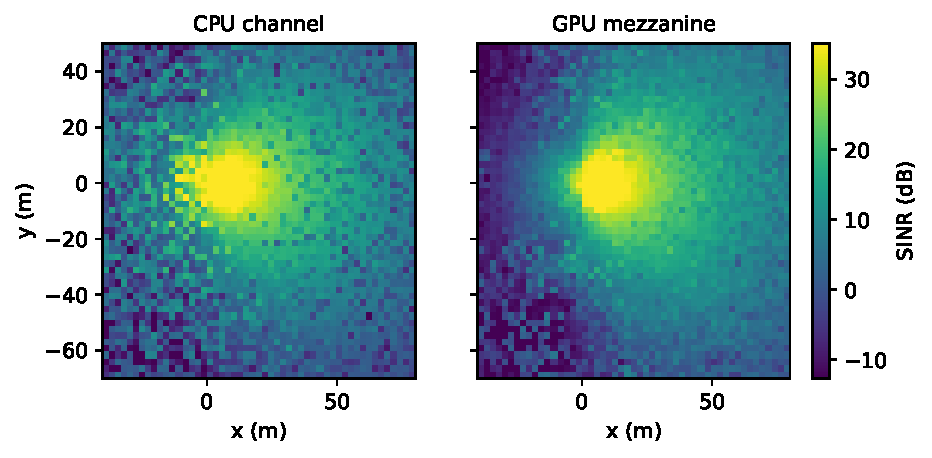
\includegraphics[width=0.94\textwidth]{fig-rem.pdf}
  \vspace{0.1em}
  \begin{itemize}\small
    \item Same coverage \alert{structure}; median SINR within \alert{0.3 dB}
          (CPU 7.55, GPU 7.27).
    \item The fine speckle is \alert{per-pixel fast fading} (a different RNG
          draw), not a scaling error -- the seed-noise spread we expect.
  \end{itemize}
\end{frame}

%==============================================================================
\begin{frame}{The cross-check paid off: it found real bugs}
  Comparing two engines is a powerful way to catch mistakes \alert{in both}.
  \begin{itemize}
    \item \textcolor{cpuCol}{\textbf{CPU bug ($\sim$30 dB!)}}: with a directional
          antenna, its $\sim$30 dB back-null was applied to the wrong rays on
          ``reversed'' links -- so \alert{every} coverage-map pixel was $\sim$30 dB
          too weak. Hidden for months (all unit tests used isotropic antennas).
          \textbf{Fixed.}
    \item \textcolor{cpuCol}{\textbf{CPU bug}}: a beam-scan copy-paste -- the
          phone's vertical scan stepped by the \emph{base station's} step.
          Breaks uneven arrays. \textbf{Fixed.}
    \item \textcolor{gpuCol}{\textbf{GPU, now fixed}}: reads the real 3GPP
          \emph{indoor and outdoor} element patterns (was outdoor-only); the
          apparent ``too-smooth'' GPU fading was largely the CPU back-null bug
          above, not a GPU defect.
  \end{itemize}
\end{frame}

%==============================================================================
\begin{frame}{Speedup}
  \begin{columns}[c]
  \begin{column}{0.5\textwidth}
    \centering
    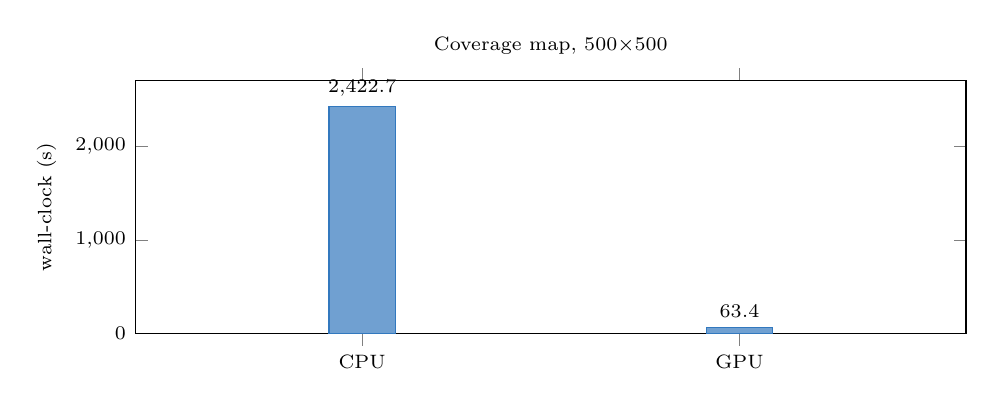
\begin{tikzpicture}
    \begin{axis}[
      ybar, width=\textwidth, height=4.8cm, bar width=24pt,
      ymin=0, ymax=2700, ylabel={wall-clock (s)}, ylabel style={font=\scriptsize},
      symbolic x coords={CPU,GPU}, xtick=data,
      nodes near coords, nodes near coords style={font=\scriptsize},
      tick label style={font=\scriptsize},
      title={Coverage map, 500$\times$500}, title style={font=\scriptsize},
      enlarge x limits=0.6,
    ]
      \addplot[fill=gpuCol!70,draw=gpuCol] coordinates {(CPU,2422.7) (GPU,63.4)};
    \end{axis}
    \end{tikzpicture}\\[-0.2em]
    {\scriptsize $\approx$\,\textbf{38$\times$} faster (2422.7 s $\to$ 63.4 s).}
  \end{column}
  \begin{column}{0.48\textwidth}
    \begin{itemize}\small
      \item Coverage maps (REM): \alert{23--38$\times$}.
      \item Channel-only benchmark: \alert{$\sim$10$\times$}, up to
            \alert{$\sim$150$\times$} with multi-slot look-ahead.
      \item Full 5G system sims: \alert{$\sim$2.3--3.1$\times$} (DenseAmimo MIMO,
            10--100\,MHz, full channel $+$ max interference) -- capped by the
            un-offloadable stack (Amdahl, next slides).
    \end{itemize}
    \vspace{0.3em}
    \begin{block}{Honest caveat}
      The tiny ``which cell do I attach to?'' sweep is dispatch-bound and is
      \alert{still faster on the CPU} (21.6 s vs 30.2 s). GPU wins on the
      \alert{heavy, many-link} work.
    \end{block}
  \end{column}
  \end{columns}
\end{frame}

%==============================================================================
\begin{frame}{Speedup grows with bandwidth, then plateaus}
  \begin{columns}[c]
  \begin{column}{0.5\textwidth}
    \centering
    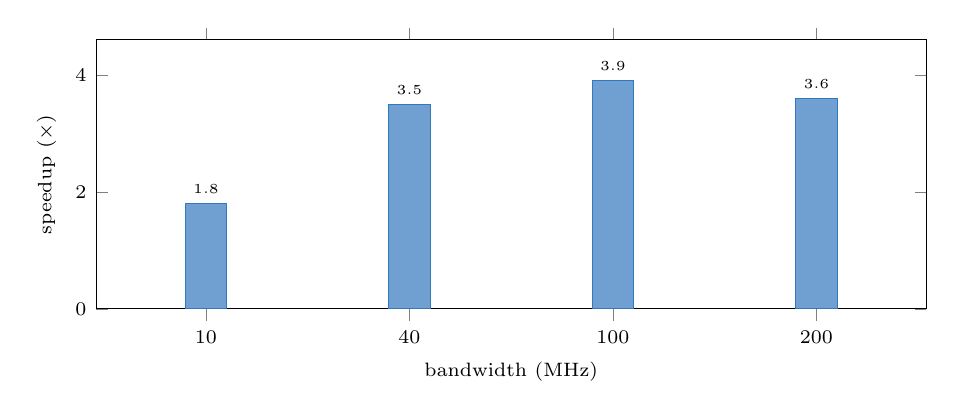
\begin{tikzpicture}
    \begin{axis}[
      ybar, width=\textwidth, height=5.0cm, bar width=15pt,
      ymin=0, ymax=4.6, ylabel={speedup ($\times$)}, ylabel style={font=\scriptsize},
      symbolic x coords={10,40,100,200}, xtick=data,
      xlabel={bandwidth (MHz)}, xlabel style={font=\scriptsize},
      nodes near coords, nodes near coords style={font=\tiny},
      tick label style={font=\scriptsize}, enlarge x limits=0.18,
    ]
      \addplot[fill=gpuCol!70,draw=gpuCol] coordinates {(10,1.8)(40,3.5)(100,3.9)(200,3.6)};
    \end{axis}
    \end{tikzpicture}
  \end{column}
  \begin{column}{0.48\textwidth}\small
    \centering
    \begin{tabular}{rrrr}
      \toprule
      BW & CPU & GPU & speedup\\
      \midrule
      10\,MHz  & 290\,s & 163\,s & 1.8$\times$\\
      40\,MHz  & 535\,s & 152\,s & 3.5$\times$\\
      100\,MHz & 355\,s & \phantom{0}92\,s & \textbf{3.9$\times$}\\
      200\,MHz & 343\,s & \phantom{0}95\,s & 3.6$\times$\\
      \bottomrule
    \end{tabular}
    \vspace{0.6em}
    \begin{itemize}\footnotesize
      \item Wider band $=$ more subcarriers $=$ more \alert{parallel} work the
            GPU absorbs almost for free (GPU wall stays $\sim$90--160\,s).
      \item Ratio climbs to \alert{$\sim$4$\times$} then plateaus -- the
            un-offloadable stack floor (Amdahl, next).
    \end{itemize}
  \end{column}
  \end{columns}
  \vspace{0.2em}
  {\scriptsize DenseA, ring-1, omni BF, 100\,ms channel update;
   10/40\,MHz at numerology~0, 100/200\,MHz at numerology~1/2.}
\end{frame}

%==============================================================================
\begin{frame}{Same kernels, different silicon: Windows/Radeon vs Apple M4 Pro}
  \centering
  {\footnotesize The \alert{identical} WebGPU mezzanine, re-measured on a second
   platform -- same scenario, same SINR, only the OS/CPU/GPU change.}
  \vspace{0.4em}

  {\small
  \setlength{\tabcolsep}{4.5pt}
  \begin{tabular}{llll rrr c}
    \toprule
    OS & CPU & GPU \scriptsize(WebGPU) & BW & CPU\,s & GPU\,s & +batch\,s & speedup\\
    \midrule
    \rowcolor{cpuCol!8}
    \textcolor{cpuCol}{\textbf{Win 11}} & Ryzen 9 7940HS & Radeon 780M & 10 & 196.0 & 84.0 & 84.0 & \textbf{2.33$\times$}\\
    \rowcolor{gpuCol!8}
    \textcolor{gpuCol}{\textbf{macOS 26}} & Apple M4 Pro & M4 Pro 16-core & 10 & 140.3 & 41.7 & 41.9 & \textbf{3.36$\times$}\\
    \rowcolor{gpuCol!8}
    \textcolor{gpuCol}{\textbf{macOS 26}} & Apple M4 Pro & M4 Pro 16-core & 40 & 142.0 & 41.9 & 42.8 & \textbf{3.39$\times$}\\
    \bottomrule
  \end{tabular}}
  \\[0.3em]
  {\scriptsize DenseAmimo, ring-1, MIMO $+$ batched covariance, 100\,ms channel
   update, num.~0 (5/10/20/40\,MHz). Win~11 row $=$ Radeon 780M (RDNA\,3);
   macOS rows $=$ Apple M4 Pro (16-core GPU, Dawn $\to$ Metal).}
  \vspace{0.2em}
  \begin{columns}[T]
  \begin{column}{0.5\textwidth}
    \begin{block}{Apple silicon wins on both wall and ratio}\footnotesize
      M4 Pro beats the 780M box on \alert{every} axis -- CPU \alert{140 vs 196\,s},
      GPU \alert{42 vs 84\,s}, and a \alert{higher speedup} too
      (\alert{3.4$\times$} vs 2.3$\times$): faster CPU baseline \emph{and} a 16-core
      GPU that clears the channel work in well under half the time.
    \end{block}
  \end{column}
  \begin{column}{0.48\textwidth}
    \begin{block}{Wider band is still free}\footnotesize
      On the M4 the GPU wall is \alert{flat 10$\to$40\,MHz} (41.7 $\to$ 41.9\,s):
      the extra subcarriers vanish into the 16-core GPU -- the same
      ``parallel-for-free'' story, on Metal instead of D3D12.
    \end{block}
  \end{column}
  \end{columns}
\end{frame}

%==============================================================================
\begin{frame}{Pushing further: the last CPU-only piece}
  Channel + beamforming now live on the GPU. \alert{MIMO adds one more cost}:
  the \alert{interference covariance} -- each receiver sums the interference from
  every other cell, $\sum_i \mathbf{H}_i\mathbf{H}_i^{H}$ per subcarrier.
  \vspace{0.5em}
  \begin{columns}[T]
  \begin{column}{0.5\textwidth}
    \begin{block}{Why it resists the GPU}
      Thousands of \alert{tiny} per-receiver sums -- each too small to beat a GPU
      dispatch on its own (the attach-sweep problem again). One-at-a-time on the
      GPU is \alert{slower} than the CPU.
    \end{block}
  \end{column}
  \begin{column}{0.48\textwidth}
    \begin{block}{Fix: batch a whole slot}
      Defer every receiver's covariance to one \alert{end-of-slot flush} and run
      them \alert{all in a single GPU pass}. \alert{Byte-identical} SINR +
      throughput, run-to-run deterministic.
    \end{block}
  \end{column}
  \end{columns}
  \vspace{0.3em}
  {\small Recovers the MIMO penalty where it bites -- \alert{$\sim$1.2$\times$} at
  100\,MHz, where the covariance is a real slice of the wall.}
\end{frame}

%==============================================================================
\begin{frame}{What each mode runs where -- and what it costs}
  \centering
  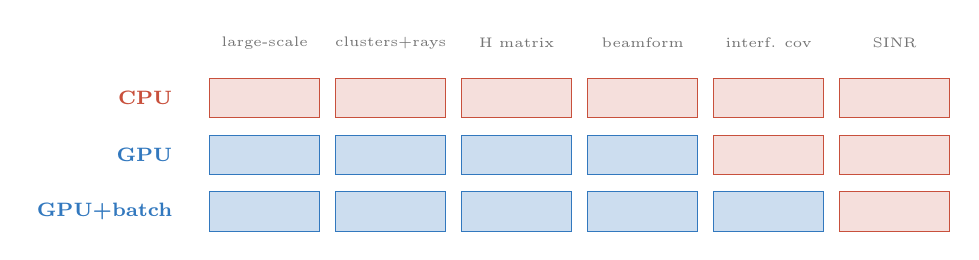
\begin{tikzpicture}[font=\tiny,
      g/.style={draw,thin,minimum height=5mm,minimum width=14mm,fill=gpuCol!25,draw=gpuCol},
      c/.style={draw,thin,minimum height=5mm,minimum width=14mm,fill=cpuCol!18,draw=cpuCol},
      rl/.style={anchor=east,font=\scriptsize}]
    % stage headers (once, on top)
    \foreach \i/\t in {0/large-scale,1/clusters+rays,2/H matrix,3/beamform,4/{interf. cov},5/SINR}
       \node[font=\tiny,text=black!55] at (\i*1.6,0.7) {\t};
    % CPU: everything on CPU, one link at a time
    \node[rl] at (-1.05,0) {\textbf{\textcolor{cpuCol}{CPU}}};
    \foreach \i in {0,...,5} \node[c] at (\i*1.6,0) {};
    % GPU (MEZ_USE_GPU): channel + beamforming on GPU; covariance + SINR on CPU
    \node[rl] at (-1.05,-0.72) {\textbf{\textcolor{gpuCol}{GPU}}};
    \foreach \i in {0,...,3} \node[g] at (\i*1.6,-0.72) {};
    \foreach \i in {4,5}     \node[c] at (\i*1.6,-0.72) {};
    % GPU+batch: + interference covariance batched on GPU
    \node[rl] at (-1.05,-1.44) {\textbf{\textcolor{gpuCol}{GPU+batch}}};
    \foreach \i in {0,...,4} \node[g] at (\i*1.6,-1.44) {};
    \node[c] at (5*1.6,-1.44) {};
  \end{tikzpicture}
  \\[0.2em]
  {\scriptsize \textcolor{gpuCol}{$\blacksquare$ on GPU}\quad
   \textcolor{cpuCol}{$\blacksquare$ on CPU}\quad--\quad
   ``batch'' defers each receiver's covariance to one end-of-slot GPU dispatch.}
  \vspace{0.35em}

  {\small
  \begin{tabular}{lccc}
    \toprule
    Mode & on GPU & \multicolumn{2}{c}{DenseAmimo ring1 wall (speedup)}\\
    \cmidrule(lr){3-4}
         &        & 10\,MHz & 100\,MHz\\
    \midrule
    CPU                         & --                    & 196\,s (1.0$\times$) & 786\,s (1.0$\times$)\\
    \code{MEZ\_USE\_GPU}        & channel $+$ beamform  & 84\,s (2.3$\times$)  & 297\,s (2.6$\times$)\\
    \;$+$ batch \emph{(default)} & $+$ interf.\ covariance & 84\,s (2.3$\times$) & \textbf{251\,s (3.1$\times$)}\\
    \;$+$ skip-matcopy          & drops H read-back$^\dagger$ & 84\,s & --\\
    \bottomrule
  \end{tabular}}
  \\[0.25em]
  {\scriptsize $^\dagger$ skip-matcopy reuses the first H -- \alert{wrong for beam-sweeping};
   the only flag with a real drawback, so \alert{opt-in}.}
\end{frame}

%==============================================================================
\begin{frame}{Where the time goes -- and why speedup has a ceiling}
  \centering
  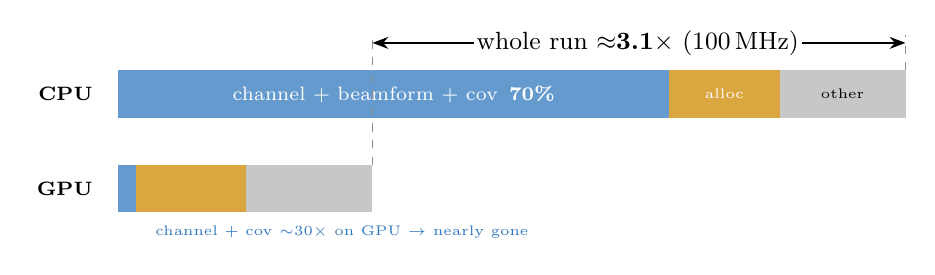
\begin{tikzpicture}[x=1mm,y=1mm,font=\scriptsize]
    % --- CPU bar: full wall normalised to 100 (DenseAmimo, 100 MHz) ---
    \node[anchor=east] at (-2,6) {\textbf{CPU}};
    \fill[gpuCol!75]  (0,3)  rectangle (70,9);
    \fill[warnCol!85] (70,3) rectangle (84,9);
    \fill[black!22]   (84,3) rectangle (100,9);
    \node[white] at (35,6) {channel + beamform + cov \,\textbf{70\%}};
    \node[white,font=\tiny] at (77,6) {alloc};
    \node[font=\tiny] at (92,6) {other};
    % --- GPU+batch bar: the 70% collapses (~30x), the 30% floor stays ---
    \node[anchor=east] at (-2,-6) {\textbf{GPU}};
    \fill[gpuCol!75]  (0,-9)    rectangle (2.3,-3);  % channel residual = 70/~30
    \fill[warnCol!85] (2.3,-9)  rectangle (16.3,-3); % alloc 14
    \fill[black!22]   (16.3,-9) rectangle (32.3,-3); % other 16
    \node[gpuCol,font=\tiny,anchor=west] at (3.5,-11.5)
        {channel $+$ cov $\sim$30$\times$ on GPU $\to$ nearly gone};
    % --- speedup bracket ---
    \draw[dashed,black!45] (100,9)--(100,13.5);
    \draw[dashed,black!45] (32.3,-3)--(32.3,13.5);
    \draw[{Stealth[length=2mm]}-{Stealth[length=2mm]},thick] (32.3,12.5)--(100,12.5);
    \node[fill=white,inner sep=1pt,font=\small] at (66,12.5) {whole run $\approx$\textbf{3.1$\times$} (100\,MHz)};
  \end{tikzpicture}
  \vspace{0.2em}
  \begin{columns}[T]
  \begin{column}{0.5\textwidth}
    \begin{block}{Amdahl's law}\small
      Make the 70\% \alert{infinitely fast} and the run still only gets
      $100/30\!\approx\!$\alert{3.3$\times$}: the un-offloadable \alert{30\%}
      (allocation + protocol stack) is the ceiling.
    \end{block}
  \end{column}
  \begin{column}{0.48\textwidth}
    \begin{block}{So why does REM hit 38$\times$?}\small
      A coverage map is \alert{almost all channel} -- almost no floor -- so the
      \alert{same kernels} give \alert{$\sim$38$\times$}. Full sims carry the
      un-offloadable stack; channel-heavy ones (big arrays, wide BW) climb higher.
    \end{block}
  \end{column}
  \end{columns}
\end{frame}

%==============================================================================
\begin{frame}[standout]
  \centering
  The 5G channel is billions of tiny matrix products.\\
  We moved them to the GPU -- same physics,\\ up to $\sim$38$\times$ faster.\\[0.6em]
  {\normalsize Thank you -- questions?}
\end{frame}

\end{document}
